Jest to biblioteka oparta o język JavaScript. Pozwala na tworzenie złożonych aplikacji webowych składających się z szerokeij listy komponentów.
Oparta jest o architekturę MVVM(ModelView View Model).
Znaczącym plusem jaki posiada ta biblioteka jest jej intuicyjność i łatwość w dostarczeniu gotowych rozwiązań.
Stale zyskuje na populaności poszerzając listę swoich zwolenników (rys. \ref{fig:vue}), oraz ilość biblotek rozszerzającyh.

\begin{figure}[!ht]
    \centering
    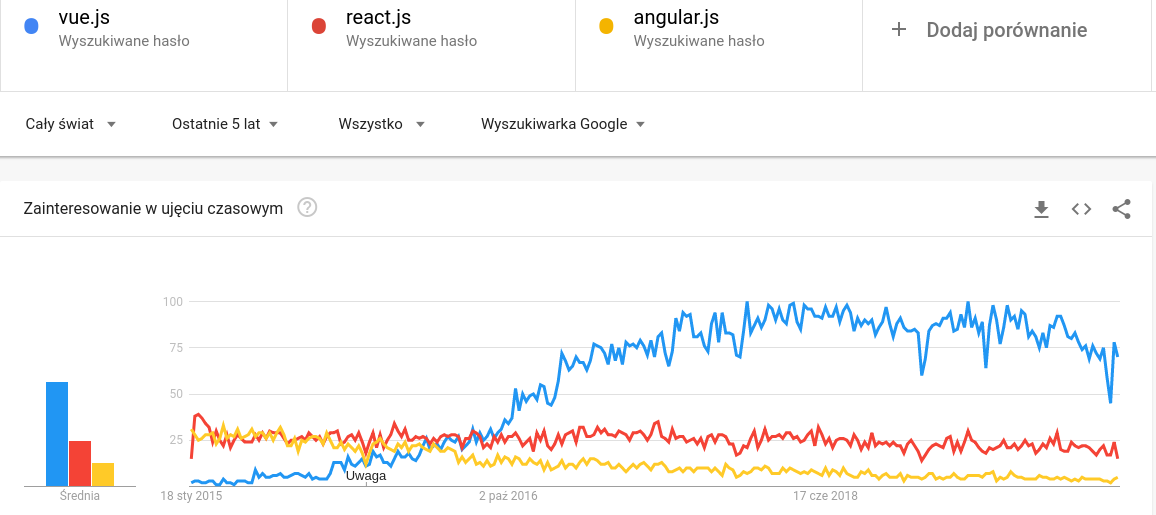
\includegraphics[width=6in]{images/vue.png}
    \caption{Popularność 3 największy frameworków JavaScript na podstawie Google Trends \label{fig:vue}}
\end{figure}